\section{\LARGE $e^x$}\label{section:exp}

We have a nice series for $e^x$ that converges quickly. In
Figure~\ref{figure:exp}, we use our expansion to $10$ terms and plot for
$e^x, x=0,\ldots,{10}$. We see that the approximation starts to diverge
significantly around $x = 7$. What this tells us is that $10$ terms are
insufficient for an accurate approximation, and more terms are needed.

\begin{figure}[bth]
  \begin{centering}
    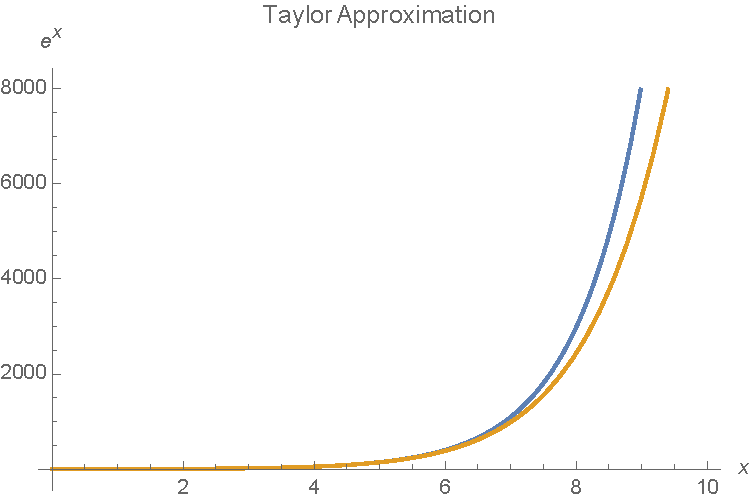
\includegraphics[width=0.65\textwidth]{images/exp.pdf}
    \caption{Comparing $e^x$ with its 10-term Taylor approximation
    centered at zero.}\label{figure:exp}
  \end{centering}
\end{figure}

\begin{figure}[bth]
  \begin{centering}
    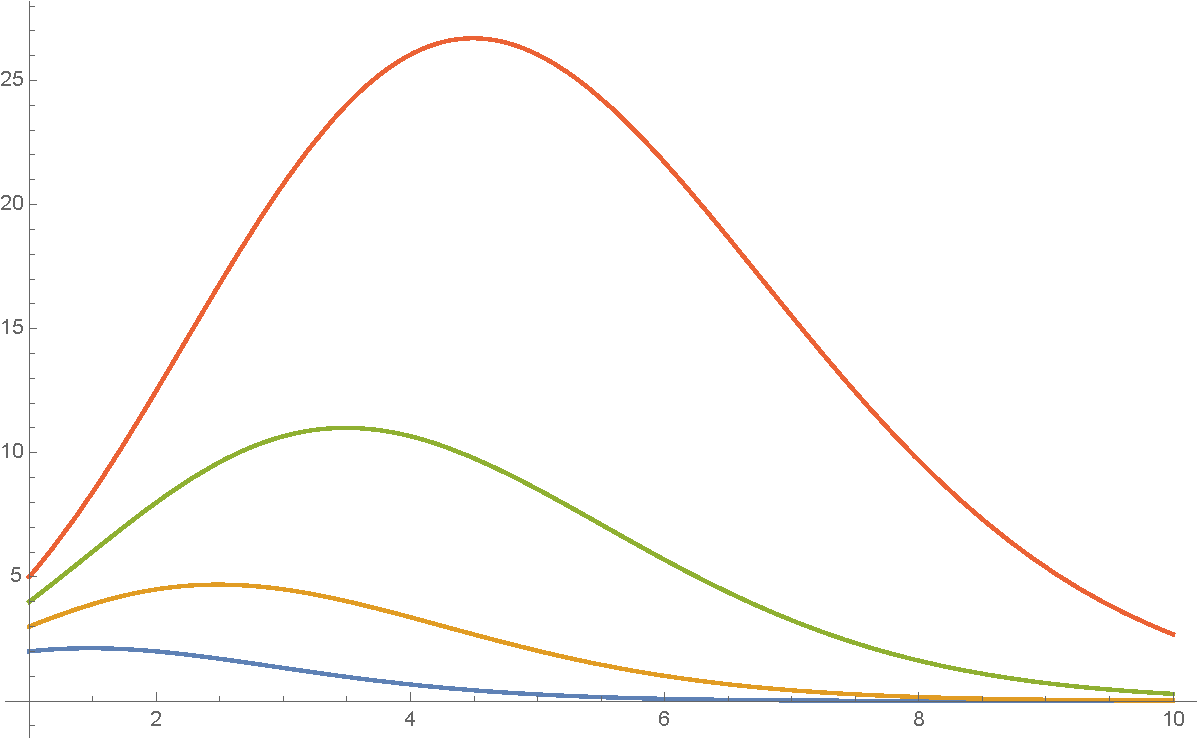
\includegraphics[width=0.75\textwidth]{images/growth.pdf}
    \caption{Comparing $\dfrac{x^k}{k!}$ for $x=2,3,4,5$.}\label{figure:growth}
  \end{centering}
\end{figure}

If we are na\"ive about computing the terms of the series we can quickly
get into trouble --- the values of $k!$ get large \emph{very quickly}.
We can do better if we observe that:
$$
\frac{x^k}{k!} = \frac{x^{k-1}}{(k-1)!} \times \frac{x}{k} .
$$

At first, that looks like a recursive definition (and in fact, you could
write it that way, but it would be wasteful). As we progress through the
computation, assume that we know the previous result. We then just have
to compute the next term and multiply it by the previous term.  At each
step we just need to compute $\frac{x}{k}$, starting with $k = 0!=1$
and multiply it by the previous value and add it
into the total. It turns into a simple \texttt{for} or \texttt{while}
loop.

We can use an $\epsilon$ (epsilon) to halt the computation since $|x^k| \ll k!$
for a sufficiently large $k$. Consider Figure \ref{figure:growth}: $x^k$
dominates briefly but is quickly overwhelmed by $k!$ and so the ratio rapidly
approaches zero. The following is an approximation of $e^x$ implemented in
Python which halts computation at a default epsilon $\epsilon = 10^{-14}$.
Make note of the efficient iterative computation of $x^k/k!$.

\begin{pylisting}{Implementation of $e^x$}
def exp(x, epsilon = 1e-14):
    trm = 1.0
    sum = trm
    k = 1
    while trm > epsilon:
        trm *= abs(x) / k
        sum += trm
        k += 1
    return sum if x > 0 else 1 / sum
\end{pylisting}

We take a different approach for $x<0$ by noting that $e^{-x} = 1/e^x$. Why is
that necessary? The series for $x\ge 0$ has all positive terms and so converges
quickly, but for $x < 0$ it is an \emph{alternating series} and converges much
more slowly. Consequently, we do a little algebra and our computation is much
more efficient.
